\documentclass[12pt,twoside]{article}
%\date{}   %uncommenting this erases the date
\usepackage{graphicx}
\usepackage{amsmath}
\usepackage{amssymb}
\usepackage[square,sort,comma,numbers]{natbib}

\usepackage{verbatim}
\usepackage{floatpag}
\usepackage{subeqnarray}
\usepackage{mathrsfs}    %for special characters
\usepackage{cancel}  % to set terms in an equation to zero


\usepackage{subcaption}
\usepackage{graphicx}
\usepackage{subcaption}


\usepackage{hyperref}
\usepackage{wrapfig}

\usepackage{amsthm}

\newtheorem{theorem}{Theorem}
\newtheorem{lemma}{Lemma}
\newtheorem{prop}{Proposition}


\setlength{\textheight}     {9.0in}
\setlength{\textwidth}      {6.5in}
\setlength{\oddsidemargin}  {0.0in}
\setlength{\evensidemargin} {0.0in}
\setlength{\topmargin}      {0.0in}
\setlength{\headheight}     {0.0in}
\setlength{\headsep}        {0.0in}
\setlength{\hoffset}        {0.0in}
\setlength{\voffset}        {0.0in}
\setlength{\parindent}      {0.0in}      %starting new line at extreme left

\graphicspath{{Figures/}}

\newcommand{\norm}[1]{\left\lVert#1\right\rVert}

\usepackage{bbm}


\linespread{2}
\usepackage{times}

\newcommand{\signaturerule}{\rule{10em}{.4pt}}
\renewcommand{\arraystretch}{1.5}

\begin{document}

\title{Runge Kutta Optimizers}
\author{Raghav Singhal}
\maketitle

\begin{abstract}
We investigate a link between the most commonly used optimization
scheme, Gradient-Descent, and a well known equation, the Gradient
Flow. Using this analogy we establish a link between Optimization
and Numerical Integration of the Gradient Flow Equation, and we
then use this analogy to investigate Runge-Kutta Methods as
optimization schemes.
\end{abstract}

%!TEX root = main.tex

\section{Introduction}
Gradient Descent or Steepest Descent Flows, is a
well studied topic in Partial Differential Equations
and Differential Geometry. Given a convex functional $f$ on a
space $X$, suppose we wish to minimize $f$, then one way
to find points $x^*$ such that $\nabla f(x^*) = 0$.
Now, finding such points in directly is not feasible, hence
we look for the shortest possible path from $x_0$ to $x^*$,
which is provided by the equation $\dot{x}(t) = - \nabla f(x(t))$,
with $x(0)=x_0$. This is fairly simple to work out in a
finite-dimensional Hilbert Space but can also be implemented
in Infinite-dimensional Space. For instance, the heat equation
can be seen as gradient flow in the Hilbert Space
$L_2(\mathbb{R}^{n})$, $u_t = \frac{\partial}{\partial u} f(u)$,
where $f(u) = \frac{1}{2} \int |\nabla u|^{2} $.
\\
\\
Now, Gradient Flow is widely used as a continuous
approximation of the Gradient Descent Method. The
analogy can be made formal by noticing that Gradient
Descent is Euler's Method to numerically solve Gradient Descent.
\\
\\
These two fields have different goals, in Optimization
the goal is to seek the minimizer of a function or in
other words, it focuses on the infinite time horizon.
In numerical analysis, the focus is on finite-time
horizon, $[0, T_{\max}]$ and to maintain consistency
and not accumulate too much error.
\\
\\
This connection was also established by Scieur et al
in \cite{integration}, where they show that accelerated
methods are instances of multi-step methods which
integrate the Gradient Flow Equation. The idea of using
differential equations to model optimization methods
has gained prominence lately, recently \cite{su} used a
second-order differential equation to model Nesterov's
Accelerated Gradient Descent. This approach however works
backwards, that is it uses the optimization scheme to
obtain a second order differential equation in the limit,
\cite{integration} however analyze Nesterov's Accelerated
Gradient Descent as a linear multi-step scheme.
\\
\\
Gradient Flow is the bridge between numerical integration
and optimization, and in \cite{integration} they used
concepts from numerical integration to show convergence
and other properties of optimization schemes. They particularly
use linear multi-step methods but in this work, we use
intermediate step methods to integrate the gradient flow
equation. The most famous family of intermediate step
methods, or half-step methods as they are commonly known,
is the Runge-Kutta Family. Here we show the performace of
half-step methods as optimization schemes.

%%% Local Variables:
%%% mode: latex
%%% TeX-master: "main"
%%% End:

%!TEX root = main.tex
% \section{Gradient Flow}
\section{Gradient Flow}
Suppose $f$ is a $\beta$-smooth and $\alpha$-Strongly
Convex function. Then gradient flow for $f$ is defined as
\begin{align}\label{grad flow}
\dot{x}(t) = - \nabla f(x(t)), \qquad x(0) = x_{0}
\end{align}
Now, as $f$ is $\beta$-smooth, we can guarantee that a
solution exists and is unique, and as $f$ is $\alpha$-Strongly
Convex, we can establish that all solutions converge to
the same equilibrium point, $x^{*}$, this equilibrium
point is the unique global minimum of $f$. \\
\\
Now, we list the two propositions that motivated our
study of numerical integration schemes for the gradient
flow equation.
\begin{prop}
  Let $x_{1}(t), x_{2}(t)$ be two solution trajectories
  of the gradient flow equation \eqref{grad flow}, then
  the following holds:
\begin{align*}
\norm{x_{1}(t) - x_{2}(t)}^{2} \leq e^{-2 \mu t} \norm{x_{1}(0) - x_{2}(0)}^{2}
\end{align*}
\end{prop}
\begin{proof}
Let $\mathcal{L}(t) = \norm{x_{1}(t) - x_{2}(t)}^{2}$, then note that
\begin{align*}
\frac{d}{dt}\mathcal{L}(t) &= 2 \langle x_{1}(t) - x_{2}(t), \dot{x_{1}}(t) - \dot{x_{2}}(t)  \rangle  \\
&= 2 \langle x_{1}(t) - x_{2}(t), -\nabla f(x_{1}(t)) + \nabla f(x_{2}(t))  \rangle  \\
& \leq - 2 \mu \mathcal{L}(t)
\end{align*}
which implies $\mathcal{L}(t) \leq e^{-2 \mu t} \mathcal{L}(0) = e^{-2 \mu t} \norm{x_{1}(0) - x_{2}(0)}^{2} $.
\end{proof}
This proposition states that any solution trajectory
of the gradient flow equation \eqref{grad flow} will
converge to the same point over time, and we show that
this point is the global minimum of $f$.
\begin{prop}
  Let $f$ be $\beta$-smooth and $\alpha$-Strongly Convex
  and $x^{*}$ is the global minimum of $f$, then the
  solution trajectory of gradient flow \eqref{grad flow} satisfies:
\begin{align*}
f(x(t)) - f(x^{*}) \leq e^{-2 \mu t} \big( f(x(0)) - f(x^{*}) \big)
\end{align*}
\end{prop}
\begin{proof}
Note that
\begin{align*}
\frac{d}{dt} \big( f(x(t)) - f(x^{*}) \big) &= \langle \nabla f(x(t)), \dot{x(t)} \rangle \\
&= - \norm{\nabla f(x(t))}^{2}
\end{align*}
Now, as $f$ is strongly convex,
\begin{align*}
f(x) - f(x^{*}) \leq \frac{1}{2 \mu} \norm{\nabla f(x)}^{2}
\end{align*}
which then implies
\begin{align*}
\frac{d}{dt} \big( f(x(t)) - f(x^{*}) \big) = -2 \mu \big( f(x(t)) - f(x^{*}) \big)
\end{align*}
Hence, $f(x(t)) - f(x^{*}) \leq e^{-2 \mu t} \big( f(x(0)) - f(x^{*}) \big)$.
\end{proof}

These two propositions motivated us to consider
numerical integration techniques for the gradient flow equation.

%%% Local Variables:
%%% mode: latex
%%% TeX-master: "main"
%%% End:

%%% Local Variables:
%%% mode: latex
%%% TeX-master: "main"
%%% End:

\section{Integration Schemes}
Schur et al \cite{integration} show that acceleration
techniques like Nesterov's accelerated gradient descent
can be seen as particular instances of multi-step methods,
popular techniques for numerical integration. Suppose we
wish to solve \eqref{grad flow} over the interval $[0, T]$,
then we discretize the solution trajectory as
$ \{ x_{1}, \dots x_{K} \} \sim \{ x(t_{1}), \dots, x(t_{k}) \} $,
where $t_0 = 0$ and $t_{k} = t_{k - 1} + \eta$ and $\eta$ is
the step size. This step size is called the learning rate in
the optimization community, and we choose it such that
$x_k \sim x(t_{k})$. Now, linear multi-step schemes are defined
as those methods which use the previous points and the derivative
values at the previous point to construct a new solution, more
precisely a linear $s$-step method is defined as follows:
\begin{align*}
  x_{k + s} = \sum_{i = 0}^{s - 1} a_{i} x_{k + i} +
  \eta \sum_{i = 0}^{s} b_{i} g(x_{k + i})
\end{align*}
where we are solving the equation $\dot{x}(t) = g(x(t))$.
If $b_{s} \neq 0$ then the above method becomes an implicit
method and if $b_{s} = 0$, then it is known as an explicit
method. A lot of current optimization schemes and acceleration
schemes rely on this technique. These techniques were invented
in order to tackle several issues like stiffness,
stability, error control, etc.
\\
\\
The focus of this work is analyzing the Runge-Kutta family,
which is a family of intermediate-step methods, that is to
get to point $x_{k + 1}$ from $x_{k}$, they use points
which are not part of the solution trajectory we finally
obtain. More formally, an $s$-step Runge Method is defined as
\begin{align*}
x_{k + 1} &= x_{k} + \eta \sum_{i = 1}^{s} c_{i} k_{i}, \quad \text{where} \\
k_{1} &= g(x_{k}) \\
k_{2} &= g(x_{k} + \eta a_{2, 1}k_{1}) \\
k_{s} &= g(x_{k} + \eta \sum_{i=1}^{s} a_{s, i} k_{i})
\end{align*}
Now, Runge-Kutta methods have to satisfy
$\sum_{j=1}^{i-1}a_{i, j} = c_{i}$ for all $i = 2, \dots, s$.
These requirements are imposed so that the method has an
error of order $p$, that is the local truncation error is
$\mathcal{O}(\eta^{p + 1})$ and a global error of
$\mathcal{O}(\eta^{p})$. The local truncation error,
$\epsilon(x_k)$, is defined as
\begin{align*}
\epsilon(x_k) = x_k - x(t_k)
\end{align*}
assuming the previous solutions $x_1, \dots, x_{k - 1}$
were exact so that $x_{k - 1} = x(t_{k - 1})$.
\\
\\
The main motivation behind explicit Runge-Kutta
methods is to use a quadrature scheme for the following problem:
\begin{align*}
x(t_{k + 1}) &= x(t_{k}) + \int_{t_k}^{t_{k + 1}} g(x(s)) ds \\
&= x(t_{k}) + \eta \int_{0}^{1}g(x(t_{k} + \eta s) ds, \quad \text{ which can be approximated as} \\
x_{k + 1} &= x_k + \eta \sum_{i = 1}^{s} b_{i} g(x_{k} + \eta c_{i})
\end{align*}
Now, as we don't have access to the intermediate
points $x(t_{k} + \eta c_i)$, we approximate by
using $x(t_k) + \eta c_i k_i$, where $k_i$ is defined above.
\\
\\
Below, we analyze two popular $2$nd-order Runge-Kutta
Method, RK2 Heun's Method,  and Ralston's Method. But
first we show a preliminary analysis on a quadratic problem
%!TEX root = main.tex



\subsubsection*{Quadratic}
The reason we focus on Runge-Kutta methods is that they perform better when dealing with stiff equations. For instance, let $f : \mathbb{R}^{d} \rightarrow \mathbb{R}$ be defined as
\begin{align*}
f(x) = \frac{1}{2} x^{T}H x  %+ c^{T}x
\end{align*}
where $H$ is positive definite, then note that $\nabla f(x) = Hx$, then gradient descent would yield
\begin{align*}
x_{k + 1} &= x_{k} - \eta H x_{k} = (I - \eta H) x_{k} \\
&= (I - \eta H)^{k} x_{0} \\
&= U (I - \eta \Lambda)^{k} U^{T} x_{0}
\end{align*}
and RK4 would yield
\begin{align*}
x_{k + 1} &= x_{k} - \frac{\eta}{6} \bigg( k_1 + 2 k_2 + 2 k_3 + k_4 \bigg) \\
&= x_k -  \frac{\eta}{6} \bigg( H x_k + 2 H (x_k - \frac{\eta}{2} H x_k ) \\
& \qquad \qquad + 2 H(x_k - \frac{\eta}{2} H (x_k - \frac{\eta}{2} H x_k )) + H(x_k - \eta H(x_k - \frac{\eta}{2} H (x_k - \frac{\eta}{2} H x_k )) ) \bigg) \\
&= x_k - \frac{\eta}{6} \bigg( 6 H x_k - 3 \eta H^{2} x_k + \frac{3 \eta^{2}}{4}H^{3}x_k - \frac{\eta^{3}}{4}H^{4} x_k  \bigg) \\
&= \bigg( I - \frac{\eta}{6} \big( 6 H - 3 \eta H^{2} + \frac{3 \eta^{2}}{4}H^{3} - \frac{\eta^{3}}{4}H^{4} \big) \bigg) x_k \\
&= U \bigg( I - \eta \Lambda +  \frac{\eta^{2}}{2} \Lambda^{2} - \frac{3 \eta^{3}}{8} \Lambda^{3} + \frac{\eta^{4}}{24} \Lambda^{4} \bigg) U^{T} x_k
\end{align*}
Now,  note that when $\eta=\frac{1}{\Lambda_{max}}$ then RK4 converges faster than Gradient Descent, but we also note that RK4 is also a corrective method and integrates much more accurately than Euler's Method.
\\
\\
In this work, however we only focus on $2$-nd order methods due to computational issues and in consideration of time.

%!TEX root = main.tex

\section{RK2 Ralston}
RK2 is a popular $2$-nd order method. The scheme for
solving $\dot{x}(t) = g(x(t))$ is defined as follows
\begin{align*}
k_{1} &= g(x_{k}) \\
k_{2} &= g(x_{k} + \eta \frac{3}{4} k_1) \\
x_{k + 1} &= x_{k} + \frac{\eta}{4} \big( k_{1} + 3 k_{2} \big)
\end{align*}
Now, if we have optimize a function, $f$, then the
RK2-Ralston Optimization Scheme is defined as follows:
\begin{align*}
  x_{k + 1} = x_{k} - \frac{\eta}{4} (\nabla f(x)
  + 3\nabla f(x - \frac{2}{3}\eta \nabla f(x)))
\end{align*}

\subsection{Strongly Convex}
\begin{theorem}\label{rk2 ralston stongly convex}
  Let $f$ be $\beta$-smooth and $\alpha$-Strongly
  Convex function. Then let $\eta = \frac{2}{\alpha + \beta}$.
Then RK-2 Ralston  satisfies:
\begin{align*}
  f(x_{k}) - f(x^{*}) \leq \frac{\beta}{2}\exp(-\frac{4 k}{\kappa + 1})
  \norm{x_{1} - x^{*}}_{2}^{2}
\end{align*}
where $\kappa = \frac{\beta}{\alpha}$ is the condition number.
\end{theorem}
\begin{proof}
  Define $r_k = \norm{x_{k} - x^{*}}$ and $F(x) =
  \nabla f(x) - 3\nabla f(x - \frac{2}{3}\eta \nabla f(x)) = k_{1} + 3k_{2}$,
\begin{align*}
\norm{x_{k + 1} - x^{*}}^{2} &= \norm{x_{k} - x^{*} - \frac{\eta}{4} F(x_k) }^{2} \\
                             &= \norm{x_{k} - x^{*}}^{2}
                               + \frac{\eta^{2}}{16}\norm{F(x_k)}^{2}
                               - \frac{\eta}{2}(x_{k} - x^{*})^{T} F(x_{k}) \\ \label{sc_rk2_ralston}
                             &= \norm{x_{k} - x^{*}}^{2}
                               + \frac{\eta^{2}}{16}\norm{k_{1}
                               + 3 k_{2}}^{2} - \frac{\eta}{2}(x_{k} - x^{*})^{T} F(x_{k}) \\
&= \norm{x_{k} - x^{*}}^{2} + \frac{\eta^{2}}{16}( \norm{k_{1}}^{2} + 9 \norm{k_{2}}^{2} + 6 k_{1}^{T} k_{2}) - \frac{\eta}{2}(x_{k} - x^{*})^{T} k_{1} - \frac{3\eta}{2}(x_{k} - x^{*})^{T}  k_{2} \\
&= \norm{x_{k} - x^{*}}^{2} + \frac{\eta^{2}}{16}( \norm{k_{1}}^{2} + 9 \norm{k_{2}}^{2} + 6 k_{1}^{T} k_{2}) - \frac{\eta}{2}(x_{k} - x^{*})^{T} k_{1} \\
& \qquad \qquad - \frac{3\eta}{2}(x_{k} - \frac{2 \eta}{3}k_{1} - x^{*})^{T}  k_{2} - \eta^{2} k_{1}^{T} k_{2} \\
& \leq \norm{x_{k} - x^{*}}^{2} + \frac{\eta^{2}}{16}( \norm{k_{1}}^{2} + 9 \norm{k_{2}}^{2}) - \frac{\eta}{2}(x_{k} - x^{*})^{T} k_{1} - \frac{3\eta}{2}(x_{k} - \frac{2 \eta}{3}k_{1} - x^{*})^{T}  k_{2}
\end{align*}
Then again by equation \eqref{coercivity}, then the above equation becomes,
\begin{align*}
r_{k + 1}^{2} & \leq r_{k}^{2} + + \frac{\eta^{2}}{16}( \norm{k_{1}}^{2} + 9 \norm{k_{2}}^{2}) - \frac{\eta}{2}(x_{k} - x^{*})^{T} k_{1} - \frac{3\eta}{2}(x_{k} - \frac{2 \eta}{3}k_{1} - x^{*})^{T}  k_{2}\\
& \leq r_{k}^{2} + \frac{\eta}{4}(\eta - \frac{2}{\alpha + \beta}) \bigg(\norm{k_{1}}^{2} + 3\norm{k_{2}}^{2} \bigg) - \frac{\eta}{2}\frac{\alpha \beta}{\alpha + \beta} \bigg(r_{k}^{2} + 3\norm{x_{k} - \frac{2 \eta}{3} k_{1} - x^{*}}^{2}\bigg)  \\
&= r_{k}^{2} - \frac{\eta}{2}\frac{\alpha \beta}{\alpha + \beta} \bigg(r_{k}^{2} + 3\norm{x_{k} - \frac{2 \eta}{3} k_{1} - x^{*}}^{2}\bigg) \\
&= r_{k}^{2} - \frac{\eta}{2}\frac{\alpha \beta}{\alpha + \beta} \bigg( r_{k}^{2} + 3 r_{k}^{2} + \frac{4 \eta^{2}}{3} \norm{\nabla f(x_k)}^{2} - 4 \eta (x_{k} - x^{*})^{T} \nabla f(x_{k}) \bigg) \\
&=  \bigg( 1 -  \frac{2 \eta \alpha \beta}{\alpha + \beta} \bigg) r_{k}^{2} - \frac{\eta}{2}\frac{\alpha \beta}{\alpha + \beta} \bigg( \frac{4 \eta^{2}}{3} \norm{\nabla f(x_k)}^{2} - 4 \eta (x_{k} - x^{*})^{T} \nabla f(x_{k}) \bigg) \\
& \leq \bigg(\frac{\kappa - 1}{\kappa + 1}\bigg)^{2} r_{k}^{2} %- 2 \eta^{2} \frac{\alpha \beta}{\alpha + \beta} \bigg( \frac{ \eta}{3} \norm{\nabla f(x_k)}^{2} -  (x_{k} - x^{*})^{T} \nabla f(x_{k}) \bigg)
\end{align*}
% Now, as $f$ is $\alpha$-Strongly convex and $\beta$-Smooth, we can show that
% \begin{align*}
% &(\nabla f(x) - \nabla f(y))^{T} (x - y)  \leq \frac{1}{\alpha}\norm{\nabla f(x) - \nabla f(y)}^{2} \\
% & \text{Use this along with \eqref{coercivity}}
% \end{align*}


\end{proof}


\subsection{Convex}
\begin{theorem}\label{rk2 ralston convex}
Let $f: \mathbb{R}^{n} \rightarrow \mathbb{R}$ be convex and $\beta$-smooth, then RK2-Ralston with $\eta = \frac{2}{\beta}$ satisfies the following:
\begin{align}
f(x_{k}) - f(x^{*}) \leq  \frac{4}{3} \frac{\norm{x_{1} - x^{*}}^{2}}{k - 1}
\end{align}
\end{theorem}

\begin{lemma} \label{lemma_2}
Let $f: \mathbb{R}^{n} \rightarrow \mathbb{R}$ be convex and $\beta$-smooth, then RK2-Ralston satisfies the following:
\begin{align*}
f(x_{k + 1}) \leq f(x_{k}) - \frac{3}{4 \beta ( k + 1)} \norm{\nabla f(x_k)}^{2}
\end{align*}
\end{lemma}

% \begin{proof}\ref{lemma_2}
% As done in the previous lemma, define $\Delta x = \nabla f(x) + 3\nabla f(x - \frac{2}{3}\eta \nabla f(x))$, then note that
% \begin{align*}
% f(x_{k + 1}) - f(x_{k}) &\leq - \frac{\eta}{4}\nabla f(x_{k})^{T} \Delta x_{k} + \frac{\eta^{2} \beta}{32} \norm{\Delta x_{k}}^{2} \\
% &= - \frac{\eta}{4}\nabla f(x_{k})^{T}( k_{1} + 3 k_{2} ) + \frac{\eta^{2} \beta}{32} \norm{ k_{1} + 3 k_{2} }^{2} \\
% &= - \frac{\eta}{4} ( \norm{k_{1}}^{2} + 3 k_{1}^{T} k_{2} ) + \frac{\eta^{2} \beta}{32} ( 2 \norm{k_{1}}^{2} + 18 \norm{k_{2}}^{2} ) \\
% &= - \frac{\eta}{4} \norm{k_{1}}^{2} \bigg( 1 - \frac{\eta \beta}{4} \bigg)
%  - \frac{3 \eta}{4} k_{1}^{T} k_{2} + \frac{9 \eta^{2} \beta}{16}\norm{k_{2}^{2}}
% \end{align*}
% Now, note that
% \begin{align*}
% & k_{1}^{T} k_{2}  \sim = \norm{k_{1}}^{2} - \eta \\
% \norm{k_{2}}^{2} &= \norm{k_{1}}^{2} + \frac{4 \eta^{2}}{9} \norm{ \nabla^{2} f(x) k_{1}} -  \frac{4 \eta}{3} k_{1}^{T} \nabla^{2} f(x) k_{1}
% \end{align*}

% \end{proof}

\begin{proof}(Lemma \ref{lemma_2})
Let $\Delta x =  \frac{1}{2\beta}(k_1 + 3k_2)$, where $\eta = \frac{2}{\beta}$ then note that
\begin{equation}
\begin{aligned}\label{ineq0}
f(x - \Delta x) - f(x) &\leq \nabla f(x)^T (x - \Delta x - x) + \frac{\beta}{2} || x - x - \Delta x ||^2 \\
&= -  \nabla f(x)^T ( \Delta x) + \frac{1}{16 \beta} || \Delta x ||^2 \\
&= -\frac{1}{2 \beta} \nabla  f(x)^T ( k_1 + 3k_2) + \frac{1}{16 \beta} || \Delta x ||^2 \\
&= -\frac{1}{2\beta}\nabla f(x)^T k_1 - \frac{3}{2\beta}\nabla f(x)^T k_2 + \frac{1}{16 \beta} || k_1 ||_2^2 + \frac{9}{16 \beta} || k_2 ||^2_2 + \frac{6}{16\beta}\left\langle k_1, k_2 \right\rangle \\
&= -\frac{1}{2\beta}\nabla f(x)^T k_1 +  \frac{1}{16 \beta} || k_1 ||_2^2 -  \frac{3}{2\beta}\nabla f(x)^T k_2 +  \frac{9}{16 \beta} || k_2 ||^2_2  + \frac{6}{16\beta}k_1^{T} k_2 \\
&= -\frac{7}{16 \beta}|| k_1 ||_2^2 -\frac{1}{16 \beta}k_2^T(24 \nabla f(x) - 9 k_2) + \frac{6}{16\beta}k_1^{T} k_2 \\
&= -\frac{7}{16 \beta}|| k_1 ||_2^2 - \frac{24}{16 \beta}k_2^Tk_1 + \frac{6}{16 \beta}k_1^{T} k_2 + \frac{9}{16\beta}|| k_2 ||_2^2 \\
&= -\frac{7}{16 \beta}|| k_1 ||_2^2 - \frac{18}{16 \beta} k_1^{T} k_2 + \frac{9}{16 \beta}|| k_2 ||_2^2
\end{aligned}
\end{equation}

Now, using a Taylor Series approximation for $\nabla f \big( x -  \frac{2\eta}{3}k_1 \big)$, we get that,
\begin{equation}
\begin{aligned}\label{ineq1}
\nabla f \big( x - \frac{2\eta}{3}k_1 \big) &= \nabla f(x) - \frac{2\eta}{3} \nabla^2 f(x) \nabla f(x) + \mathcal{O}( |\frac{2\eta}{3} |^2 ) \\
\implies  k_2^Tk_1 &= \nabla f \big( x - \frac{2\eta}{3}k_1 \big)^T\nabla f(x) \\
 &= \nabla f \big( x - \frac{2\eta}{3}\nabla f(x) \big)^T \nabla f(x) \\
&= || \nabla f(x) ||_2^2 - \frac{2\eta}{3} \nabla f(x)^T \nabla^2 f(x) \nabla f(x)
\end{aligned}
\end{equation}
And, using \eqref{ineq1},
\begin{equation}
\begin{aligned} \label{ineq2}
|| k_2 ||_2^2 &= ||  \nabla f(x) - \frac{2\eta}{3} \nabla^2 f(x) \nabla f(x)  ||_2^2   \\
&= || \nabla f(x)||_2^2 + \frac{4\eta}{9}||\nabla^2 f(x) \nabla f(x)  ||_2^2 - \frac{4\eta}{3} \nabla f(x)^T \nabla^2 f(x) \nabla f(x)
\end{aligned}
\end{equation}
Hence, using \eqref{ineq1} and \eqref{ineq2}
\begin{align*}
f(x - \Delta x) - f(x) & \leq  -\frac{7}{16 \beta}|| k_1 ||_2^2 - \frac{18}{16 \beta}  k_1^{T} k_2  + \frac{9}{16 \beta}|| k_2 ||_2^2 \\
&= -\frac{7}{16 \beta}|| \nabla f(x) ||_2^2 -  \frac{18}{16 \beta} || \nabla f(x) ||_2^2 + \frac{12}{16 \beta^2} \nabla f(x)^T \nabla^2 f(x) \nabla f(x) \\
&+  \frac{9}{16\beta}( || \nabla f(x)||_2^2 + \frac{4}{9\beta}||\nabla^2 f(x) \nabla f(x)  ||_2^2 - \frac{4}{3\beta} \nabla f(x)^T \nabla^2 f(x) \nabla f(x) )  \\
&= -\frac{16}{16 \beta}|| \nabla f(x)||_2^2 + \frac{1}{4 \beta^2}||\nabla^2 f(x) \nabla f(x)  ||_2^2 \\
&= -\frac{1}{\beta} || \nabla f(x)||_2^2 + \frac{1}{4 \beta^2}||\nabla^2 f(x) \nabla f(x)  ||_2^2 \\
\end{align*}
Using the lipschitz property of the Hessian of $f$, $||\nabla^2 f(x) u - \nabla^2 f(x) v||_2^2 \leq \beta || u-v ||_2^2 $, we get that,
\begin{equation}
\begin{aligned}
f(x - \Delta x) - f(x) & \leq -\frac{1}{\beta} || \nabla f(x)||_2^2 + \frac{1}{4\beta^2}||\nabla^2 f(x) \nabla f(x)  ||_2^2 \\
& \leq -\frac{4}{4\beta}|| \nabla f(x) ||_2^2 + \frac{\beta}{4 \beta^2}|| \nabla f(x) ||_2^2 \\
& = -\big( \frac{4}{4\beta} - \frac{\beta}{8\beta^2}   \big)  || \nabla f(x) ||_2^2  \\
&= -\frac{3}{4\beta} || \nabla f(x) ||_2^2
\end{aligned}
\end{equation}
\end{proof}

\begin{proof}(Theorem \ref{rk2 ralston convex})
Using Lemma 1, we have $f(x_{t+1}) - f(x_{t}) \leq -\frac{3}{4\beta}|| \nabla f(x_{t}) ||_2^2 $. Now, let $\delta_t = f(x_t) - f(x^*)$, then note that:
\begin{align*}
\delta_{t+1} \leq \delta_t - \frac{3}{4\beta}|| \nabla f(x) ||_2^2
\end{align*}
Now, by convexity of $f(x)$ we have:
\begin{align}
\delta_t &\leq \nabla f(x_t)^T (x_t - x^*) \\
 &\leq || x_t - x^* ||_2 * || \nabla f(x_t) ||_2 \\
\frac{1}{|| x_t - x^* || }\delta_t^2 & \leq  || \nabla f(x_t) ||_2^2
\end{align}

Now, note that $|| x_t - x^*||_2^2$ is decreasing, using the following inequality
\begin{align*}
\big( \nabla f(x) - \nabla f(y)  \big)^T(x-y)  \geq \frac{1}{\beta} || \nabla f(x) - \nabla f(y) ||_2^2
\end{align*}
Using the above and the fact that $\nabla f(x^*) = 0$,
\begin{align*}
|| x_{t+1} - x^* ||_2^2 &= || x_t - \Delta x_t - x^* ||_2^2 \\
&= || x_t - x^* ||_2^2 + || \Delta x_t ||_2^2 - 2 \Delta x_t^T(x_t - x^*) \\
&= || x_t - x^* ||_2^2 - \frac{1}{\beta}(k_1 + 3k_2)^T (x_t - x^*) + \frac{1}{4 \beta^2}|| k_1 + 3k_2 ||_2^2 \\
&= || x_t - x^* ||_2^2 - \frac{1}{ \beta}k_1^T (x_t - x^*) + \frac{1}{4 \beta^2}|| k_1 ||_2^2  \\
& \quad \quad \quad - \frac{3}{\beta}k_2^T (x_t - x^*) + \frac{9}{4 \beta^2}|| k_2 ||_2^2 + \frac{6}{4 \beta^2} k_1 ^T k_2 \\
&= || x_t - x^* ||_2^2 - \frac{4}{4 \beta^2}||k_1 ||_2^2 + \frac{1}{4 \beta^2}|| k_1 ||_2^2  \\
& \quad \quad \quad - \frac{12}{4 \beta^2}|k_2||_2^2 + \frac{9}{4 \beta^2}|| k_2 ||_2^2 + \frac{6}{4 \beta^2} k_1 ^T k_2 \\
&= || x_t - x^* ||_2^2 - \frac{3}{4 \beta^2}||k_1||_2^2 - \frac{3}{4 \beta^2}||k_2||_2^2 + \frac{6}{4 \beta^2} k_1 ^T k_2 \\
&= || x_t - x^* ||_2^2 -  \frac{3}{4 \beta^2}|| k_1 - k_2||_2^2  \\
& \leq || x_t - x^* ||_2^2
\end{align*}
We will show that,
\begin{align}
\delta_{t+1} \leq \delta_t - \frac{3}{4 \beta || x_1 - x^* ||_2^2} \delta_t^2
\end{align}
Now, let $\omega = \frac{3}{4 \beta   || x_1 - x^* ||_2^2}$, %then note that: (Proof in Bubek page - 269)
\begin{align*}
& \frac{1}{\delta_t} \geq \omega (t-1) \\
\implies & f(x_t) - f(x^*) \leq \frac{4}{3 \beta} \frac{ || x_1 - x^* ||_2^2}{t-1} \xrightarrow{t \to \infty} 0
\end{align*}
\end{proof}


% \subsection{Stochastic -  Strongly Convex}


%%% Local Variables:
%%% mode: latex
%%% TeX-master: "main"
%%% End:

%!TEX root = main.tex
\section{RK2 Heun}
RK2 Heun is commonly known as a predictor-corrector algorithm. It is based on Euler's Method, where like Euler's Method it uses the tangent to the function at some point to obtain the next point, however even when the step-size or the learning rate is small, the error starts to accumulate over time, however the second step is meant to act as a corrector step. The scheme is defined as follows for the equation $\dot{x}(t) = g(x(t))$
\begin{align*}
k_1 &= g(x_k) \\
k_2 &= g(x_k + \eta k1) \\
x_{k + 1} &= x_{k} + \frac{\eta}{2} \big( k_1 + k_2 \big)
\end{align*}
In other words if we wish to minimize the function $f$, then RK2 heun's method scheme is defined as follows:
\begin{equation*}
x_{k + 1} = x_{k} - \frac{\eta}{2} (\nabla f(x_k) - \nabla f(x_k - \eta \nabla f(x_k)))
\end{equation*}

\subsection{Strongly Convex}
\begin{theorem}
Let $f$ be $\beta$-smooth and $\alpha$-Strongly Convex function. Then let $\eta = \frac{4}{\alpha + \beta}$.
Then RK-2 Heun's method satisfies:
\begin{align*}
f(x_{k}) - f(x^{*}) \leq \frac{\beta}{2} \exp \bigg(- \frac{8 k}{ \kappa + 1} \bigg) \norm{x_{1} - x^{*}}^{2}
\end{align*}
where $\kappa = \frac{\beta}{\alpha}$ is the condition number.
\end{theorem}
\begin{proof}
Define $r_k = \norm{x_{k} - x^{*}}$ and $F(x) = \nabla f(x) + \nabla f(x - \eta \nabla f(x)) = k_{1} + k_{2}$, then note that
\begin{align}
\norm{x_{k + 1} - x^{*}}^{2} &= \norm{x_{k} - x^{*} - \frac{\eta}{2}F(x_{k})}^{2} \\
&= \norm{x_{k} - x^{*}}^{2} + \frac{\eta^{2}}{4}\norm{F(x_{k})}^{2} - \eta (x_{k} - x^{*})^{T} F(x_k) \\ \label{r}
& \leq \norm{x_{k} - x^{*}}^{2} + \frac{\eta^{2}}{4}(\norm{k_{1}}^{2} + \norm{k_{2}}^{2} + 4 k_{1}^{T} k_{2}) - \eta (x_{k} - x^{*})^{T} F(x_k)
\end{align}
Now, note that for $f \in \mathcal{S}_{\beta, \alpha}(\mathbb{R}^{n})$, that is $f$ is $\beta$-smooth and $\alpha$-Strongly Convex function,
\begin{align} \label{coercivity}
(\nabla f(x) - \nabla f(y))^{T}(x - y) \geq \frac{\alpha \beta}{\alpha + \beta}\norm{x - y}^{2} + \frac{1}{\alpha + \beta}\norm{\nabla f(x) - \nabla f(y)}^{2}
\end{align}
So using \eqref{coercivity}, the inequality \eqref{r} reduces to

\begin{align}
r_{k + 1}^{2} &\leq r_{k}^{2} + \frac{\eta^{2}}{4}(\norm{k_{1}}^{2} + \norm{k_{2}}^{2}) + \eta^{2}k_{1}^{T} k_{2} - \eta (x_{k} - x^{*})^{T} (k_{1} + k_{2}) \\
& = r_{k}^{2} + \frac{\eta^{2}}{4}(\norm{k_{1}}^{2} + \norm{k_{2}}^{2}) - \eta (x_{k} - x^{*})^{T} k_1 - \eta (x_{k} - \eta k_{1} - x^{*})^{T} k_2
\end{align}
Now, using \eqref{coercivity} on the last two terms yields

\begin{align*}
r_{k + 1}^{2} & \leq r_{k}^{2} + \frac{\eta^{2}}{4}(\norm{k_{1}}^{2} + \norm{k_{2}}^{2}) - \eta \frac{\alpha \beta}{\alpha + \beta}(r^{2}_k + \norm{x_{k} - \eta k_{1} - x^{*} }^{2})  \\ & \qquad \qquad \qquad \qquad -\eta \frac{1}{\alpha + \beta} (\norm{k_{1}}^{2} + \norm{k_{2}}^{2}) \text{    , using \eqref{coercivity}} \\
&= r_{k}^{2} + \frac{\eta}{4} (\eta - \frac{4}{\alpha + \beta})(\norm{k_{1}}^{2} + \norm{k_{2}}^{2})  - \eta \frac{\alpha \beta}{\alpha + \beta}(r^{2}_k + || x_{k} - x^{*} - \eta k_{1} ||^{2}) \\
&= r_{k}^{2}  - \eta \frac{\alpha \beta}{\alpha + \beta}(r^{2}_k + \norm{x_{k} - x^{*} - \eta k_{1}}^{2}) \text{    , since $\eta = \frac{4}{\beta + \alpha}$} \\
& \leq r_{k}^{2} - \eta \frac{\alpha \beta}{\alpha + \beta}(r_{k}^{2} +  \norm{x_{k} - x^{*} - \eta k_{1}}^{2}) \\
& \leq r_{k}^{2}(1 - \eta \frac{\alpha \beta}{\alpha + \beta})  -  \eta \frac{\alpha \beta}{\alpha + \beta}( \norm{x_{k} - x^{*} - \eta k_{1}}^{2})
\end{align*}
where the last two inequality follows as $\norm{x - y}^{2} \geq (\norm{x} - \norm{y})^{2}$ and as $\norm{\nabla f(x) - \nabla f(y)} \leq \beta \norm{x - y}$
\begin{align}
r_{k}^{2}&= r_{k}^{2} \bigg(1 - 4  \frac{\alpha \beta}{(\alpha + \beta)^{2}} \bigg) -  4  \frac{\alpha \beta}{(\alpha + \beta)^{2}}( \norm{x_{k} - x^{*} - \eta k_{1}}^{2})  \\
& \leq r_{k}^{2} \bigg(\frac{\beta - \alpha}{\beta + \alpha}\bigg)^{2} -  4  \frac{\alpha \beta}{(\alpha + \beta)^{2}}( \norm{x_{k} - x^{*} - \eta k_{1}}^{2})  \\
&= \bigg(\frac{\kappa - 1}{\kappa + 1}\bigg)^{2} r_{k}^{2} -  4  \frac{\alpha \beta}{(\alpha + \beta)^{2}}( \norm{x_{k} - x^{*} - \eta k_{1}}^{2}) \\
r^{2}_{k + 1} &\leq \exp \bigg(- \frac{8 k}{ \kappa + 1} \bigg) \norm{x_{1} - x^{*}}^{2}
\end{align}
where $\kappa = \frac{\beta}{\alpha}$ is known as the condition number of $f$.
\end{proof}

% Note as $f$ is $\alpha$-Strongly Convex and $\beta$-smooth, we know that $ \beta I \succeq \nabla^{2}f(x) \succeq \alpha I$, then by Taylor Series's approximation
% \begin{align*}
% k_{1}^{T} k_{2} & \sim \norm{\nabla f(x_{k})}^{2} - \eta \nabla f(x_{k})^{T} \nabla^{2} f(x_{k}) \nabla f(x_{k}) \\
% & = \norm{\nabla f(x_{k})}^{2} - \frac{4}{\alpha + \beta} \nabla f(x_{k})^{T} \nabla^{2} f(x_{k}) \nabla f(x_{k}) \geq 0
% \end{align*}

% \textbf{Impose the above condition in the theorem}


\subsection{Convex}
\begin{theorem} \label{rk2_heun_convex}
Let $f : \mathbb{R}^{n} \rightarrow \mathbb{R}^{n} $ be convex and $\beta$-smooth, then with $\eta = \frac{1}{\beta}$, RK2-Heun satisfies:
\begin{align*}
f(x_{k}) - f(x^{*}) \leq  \frac{2}{3 \beta} \frac{\norm{x_{1} - x^{*}}^{2}}{k - 1}
\end{align*}
\end{theorem}

\begin{lemma} \label{rk2_heun_convex_lemma}
Let $f : \mathbb{R}^{n} \rightarrow \mathbb{R}^{n} $ be convex and $\beta$-smooth, then with $\eta = \frac{1}{\beta}$, RK2-Heun satisfies:
\begin{align}
f(x_{k + 1}) \leq f(x_{k}) - \frac{3}{2 \beta } \norm{\nabla f(x_k)}^{2}
\end{align}
\end{lemma}

The Proof for Theorem \ref{rk2_heun_convex} follows the same steps as the proof for Rk2 Ralston convex case.
% \begin{proof}(Lemma \ref{rk2 heun convex lemma})
% % Let $\Delta x = \frac{1}{2\beta}(k_1 + k_2) $, then using Taylor Series approximation we get that:
% % \begin{equation}
% % \begin{aligned}
% % f(x - \Delta x) - f(x) &\leq \nabla f(x)^T ( - \Delta x) + \frac{\beta}{2}|| \Delta x||_2^2 \\
% % & = - \frac{1}{2\beta}\nabla f(x)^T (k_1 + k_2) + \frac{1}{8\beta}||k_1 + k_2 ||_2^2 \\
% % & = - \frac{1}{2\beta}\nabla ||f(x)||_2^2 - \frac{1}{2\beta}\nabla f(x)^T k_2 + \frac{1}{8\beta}||\nabla f(x)||_2^2 + \frac{1}{8\beta}||k_2||_2^2 + \frac{1}{2\beta}k_1^T k_2 \\
% % & = -\frac{3}{8\beta}||\nabla f(x)||_2^2 + \frac{1}{8\beta}||k_2||_2^2 \\
% % & = -\frac{3}{8\beta}||\nabla f(x)||_2^2 + \frac{1}{8\beta}||\nabla f(x)||_2^2 + \frac{1}{8\beta^2}||\nabla^2 f(x) \nabla f(x)||_2^2 \\
% % & \leq - \frac{1}{8\beta}|| \nabla f(x)||_2^2
% % \end{aligned}
% % \end{equation}
% Let $\Delta x = \frac{1}{2 \beta}(k_1 + k_2) $, then using Taylor Series approximation we get that:

% \begin{equation}
% \begin{aligned}
% f(x - \Delta x) - f(x) &\leq \nabla f(x)^T ( - \Delta x) + \frac{\beta}{2}|| \Delta x||_2^2 \\
% & = - \frac{1}{\beta}\nabla f(x)^T (k_1 + k_2) + \frac{1}{2\beta}||k_1 + k_2 ||_2^2 \\
% & = - \frac{1}{\beta}\nabla ||f(x)||_2^2 - \frac{1}{\beta}\nabla f(x)^T k_2 + \frac{1}{2\beta}||\nabla f(x)||_2^2 + \frac{1}{2\beta}||k_2||_2^2 + \frac{1}{\beta}k_1^T k_2 \\
% & \leq -\frac{1}{2\beta}||\nabla f(x)||_2^2 + \frac{1}{\beta}||k_2||_2^2 \\
% & = -\frac{1}{2\beta}||\nabla f(x)||_2^2 + \frac{1}{\beta}||\nabla f(x)||_2^2 + \frac{4}{\beta^2}||\nabla^2 f(x) \nabla f(x)||_2^2 \\
% & \leq - \frac{3}{2\beta}|| \nabla f(x)||_2^2
% \end{aligned}
% \end{equation}

% \end{proof}


% \begin{proof}
% Note that as $f$ is convex and $\beta$-smooth, it satisfies the following
% \begin{align} \label{convex_def}
% 0 \leq f(x) - f(y) \leq \nabla f(y)^{T} (x - y) + \frac{\beta}{2}\norm{x - y}^{2}
% \end{align}
% Now, a consequence of equation \eqref{convex_def} is that
% \begin{align} \label{convex_def_2}
% f(x) - f(y) \leq \nabla f(x)^{T}(x - y) - \frac{1}{2 \beta} \norm{\nabla f(x) - \nabla f(y)}^{2}
% \end{align}
% % Then note that
% % \begin{align}
% % f(x_{k}) - f(x^{*})
% % \end{align}

% Then using \eqref{convex_def} and \eqref{convex_def_2} we show that
% \begin{align*}
% f(x_{k + 1}) - f(x_{k}) & \leq \nabla f(x_{k})^{T} (x_{k + 1} - x_{k}) + \frac{\beta}{2}\norm{x_{k + 1} - x_{k}}^{2} \\
% & = -\frac{\eta}{2} \nabla f(x_{k})^{T}(k_{1} + k_{2}) + \frac{\eta^{2} \beta}{8} \norm{k_{1} + k_{2}}^{2} \\
% & = - \frac{\eta}{2} ( \norm{k_{1}}^{2} + k_{1}^{T} k_{2}) + \frac{\eta^{2} \beta}{8} ( \norm{k_{1}}^{2} + 2 k_{1}^{T} k_{2} +\norm{k_{2}}^{2})
% \end{align*}
% Now, let $\delta_{k} = f(x_{k}) - f(x^{*})$, then note that
% \begin{align*}
% %  % Use \\
% \norm{x + y}^{2} &\leq 2 \norm{x}^{2} +  2 \norm{y}^{2} \\
% &\text{Use in last equation to get rid of $k_{1}^{T} k_{2}$}
% \end{align*}

% \begin{align}
% \delta_{k + 1} & \leq \delta_{k} - \frac{\eta}{2} ( \norm{k_{1}}^{2} + k_{1}^{T} k_{2}) + \frac{\eta^{2} \beta}{8} ( \norm{k_{1}}^{2} + 2 k_{1}^{T} k_{2} +\norm{k_{2}}^{2}) \\
% & = \delta_{k} - \frac{\eta}{2}(1 - \frac{\eta \beta}{4})\norm{k_{1}}^{2} - \frac{\eta}{2} k_{1}^{T} k_{2}(1 - \frac{\eta \beta}{2}) + \frac{\eta^{2} \beta}{8} \norm{k_{2}}^{2} \\ \label{last_rk2_convex}
% & = \delta_{k} - \frac{3}{8 \beta} \norm{k_{1}}^{2} - \frac{2}{8 \beta} k_{1}^{T} k_{2} + \frac{1}{8 \beta} \norm{k_{2}}^{2}
% \end{align}

% For the last two terms in \eqref{last_rk2_convex}, we have that
% \begin{align*}
% k_{1}^{T} k_{2} &= \norm{\nabla f(x_{k})}^{2} - \frac{1}{\beta} \nabla f(x_{k})^{T} \nabla f(x_{k})^{2} \nabla f(x_{k}) \\
% &= \norm{k_{1}}^{2} - \frac{1}{\beta}k_{1} \nabla^{2} f(x_{k}) k_{1} \\
% \norm{k_{2}}^{2} &= \norm{\nabla f(x_{k}) - \frac{1}{\beta}\nabla f(x_{k})^{2} \nabla f(x_{k})}^{2} \\
% & = \norm{k_{1}}^{2} + \frac{1}{\beta^{2}}\norm{\nabla f(x_{k})^{2} k_{1}} - \frac{2}{\beta}k_{1} \nabla^{2} f(x_{k}) k_{1}
% \end{align*}
% therefore, using the above two, equation \eqref{last_rk2_convex} becomes
% \begin{align*}
% \delta_{k + 1} & \leq \delta_{k} - \frac{3}{8 \beta}\norm{k_{1}}^{2} - \frac{1}{8 \beta}\bigg( \norm{k_{1}}^{2} + \frac{1}{\beta}k_{1} \nabla^{2} f(x_{k}) k_{1} - \frac{1}{\beta^{2}} \norm{\nabla^{2} f(x_{k}) k_{1}) }^{2} \bigg) \\
% & = \delta_{k} - \frac{1}{2 \beta}\norm{k_{1}}^{2} - \frac{1}{8 \beta^{2}}\bigg( k_{1} \nabla^{2} f(x_{k}) k_{1} - \frac{1}{\beta} \norm{\nabla^{2} f(x_{k}) k_{1} }^{2} \bigg)
% \end{align*}

% \end{proof}
% % Note that for $f(x) = \frac{1}{2} x^{T} A x$, where $A$ is positive semi-definite, $ k_{1}^{T} k_{2} =\nabla f(x)^{T} \nabla f(x - \eta \nabla f(x)) \geq 0$ (\textbf{prove using Taylor Series somewhere}), something like this (also use $\norm{ \nabla f(x)}^{2} \leq \beta \norm{x}^{2}$)
% % \begin{align*}
% % k_{1}^{T} k_{2} \sim = \norm{\nabla f(x)}^{2} - \frac{1}{\beta}\nabla f(x)^{T} \nabla^{2} f(x) \nabla f(x) \geq 0
% % \end{align*}

% \subsection{Stochastic -  Strongly Convex}

%%% Local Variables:
%%% mode: latex
%%% TeX-master: "main"
%%% End:

\section{Optimization in Deep Leanrning}
Here we
%%% Local Variables:
%%% mode: latex
%%% TeX-master: "main"
%%% End:


% %!TEX root = main.tex



\subsubsection*{Quadratic}
The reason we focus on Runge-Kutta methods is that they perform better when dealing with stiff equations. For instance, let $f : \mathbb{R}^{d} \rightarrow \mathbb{R}$ be defined as
\begin{align*}
f(x) = \frac{1}{2} x^{T}H x  %+ c^{T}x
\end{align*}
where $H$ is positive definite, then note that $\nabla f(x) = Hx$, then gradient descent would yield
\begin{align*}
x_{k + 1} &= x_{k} - \eta H x_{k} = (I - \eta H) x_{k} \\
&= (I - \eta H)^{k} x_{0} \\
&= U (I - \eta \Lambda)^{k} U^{T} x_{0}
\end{align*}
and RK4 would yield
\begin{align*}
x_{k + 1} &= x_{k} - \frac{\eta}{6} \bigg( k_1 + 2 k_2 + 2 k_3 + k_4 \bigg) \\
&= x_k -  \frac{\eta}{6} \bigg( H x_k + 2 H (x_k - \frac{\eta}{2} H x_k ) \\
& \qquad \qquad + 2 H(x_k - \frac{\eta}{2} H (x_k - \frac{\eta}{2} H x_k )) + H(x_k - \eta H(x_k - \frac{\eta}{2} H (x_k - \frac{\eta}{2} H x_k )) ) \bigg) \\
&= x_k - \frac{\eta}{6} \bigg( 6 H x_k - 3 \eta H^{2} x_k + \frac{3 \eta^{2}}{4}H^{3}x_k - \frac{\eta^{3}}{4}H^{4} x_k  \bigg) \\
&= \bigg( I - \frac{\eta}{6} \big( 6 H - 3 \eta H^{2} + \frac{3 \eta^{2}}{4}H^{3} - \frac{\eta^{3}}{4}H^{4} \big) \bigg) x_k \\
&= U \bigg( I - \eta \Lambda +  \frac{\eta^{2}}{2} \Lambda^{2} - \frac{3 \eta^{3}}{8} \Lambda^{3} + \frac{\eta^{4}}{24} \Lambda^{4} \bigg) U^{T} x_k
\end{align*}
Now, if you note that $\eta=\frac{2}{\Lambda_{max}}$ then RK4 converges faster than Gradient Descent, but we also note that RK4 is also a corrective method and integrates much more accurately than Euler's Method.















% %!TEX root = main.tex

\section{Appendix}
\subsection{Proofs}



%!TEX root = main.tex
\begin{thebibliography}{9}
\bibitem{su}
 Su, Weijie, Stephen Boyd, and Emmanuel Candes. \textit{A differential equation for modeling Nesterov’s accelerated gradient method: Theory and insights}. Advances in Neural Information Processing Systems. 2014.

\bibitem{integration}
Scieur, Damien, et al. \textit{Integration Methods and Accelerated Optimization Algorithms} arXiv preprint arXiv:1702.06751 (2017).

\bibitem{nesterov}
Nesterov, Yurii. \textit{Introductory lectures on convex optimization: A basic course}. Vol. 87. Springer Science and Business Media, 2013.

\end{thebibliography}


%!TEX root=./main.tex
\section{Experiments}
\subsection{Deep Learning}

\textbf{ResNet18} -
Here we compare our optimization scheme with Stochastic Gradient Descent with momentum and learning rate decay.
\\
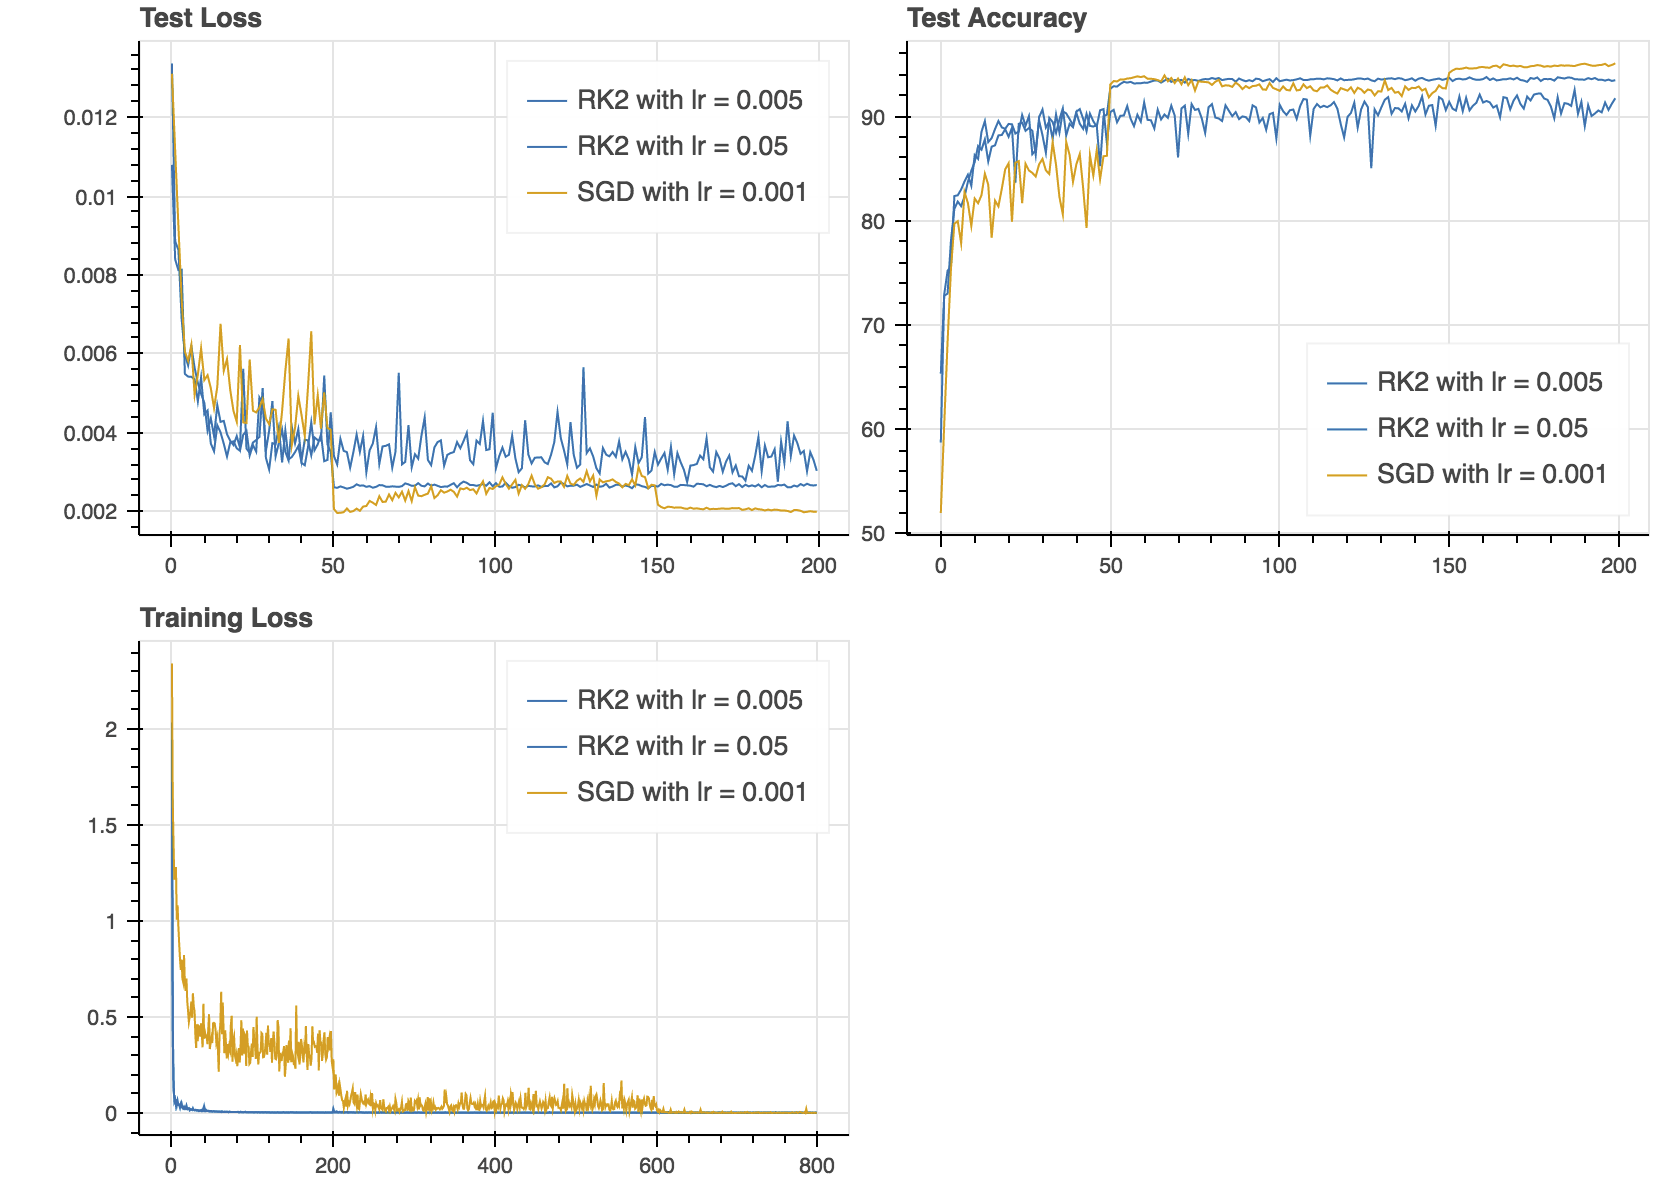
\includegraphics[scale=0.5]{cifar.png}
\textbf{WideResnet} -
Here we compare our optimization scheme, Runge-Kutta Ralston Method with Stochastic Gradient Descent.
\\
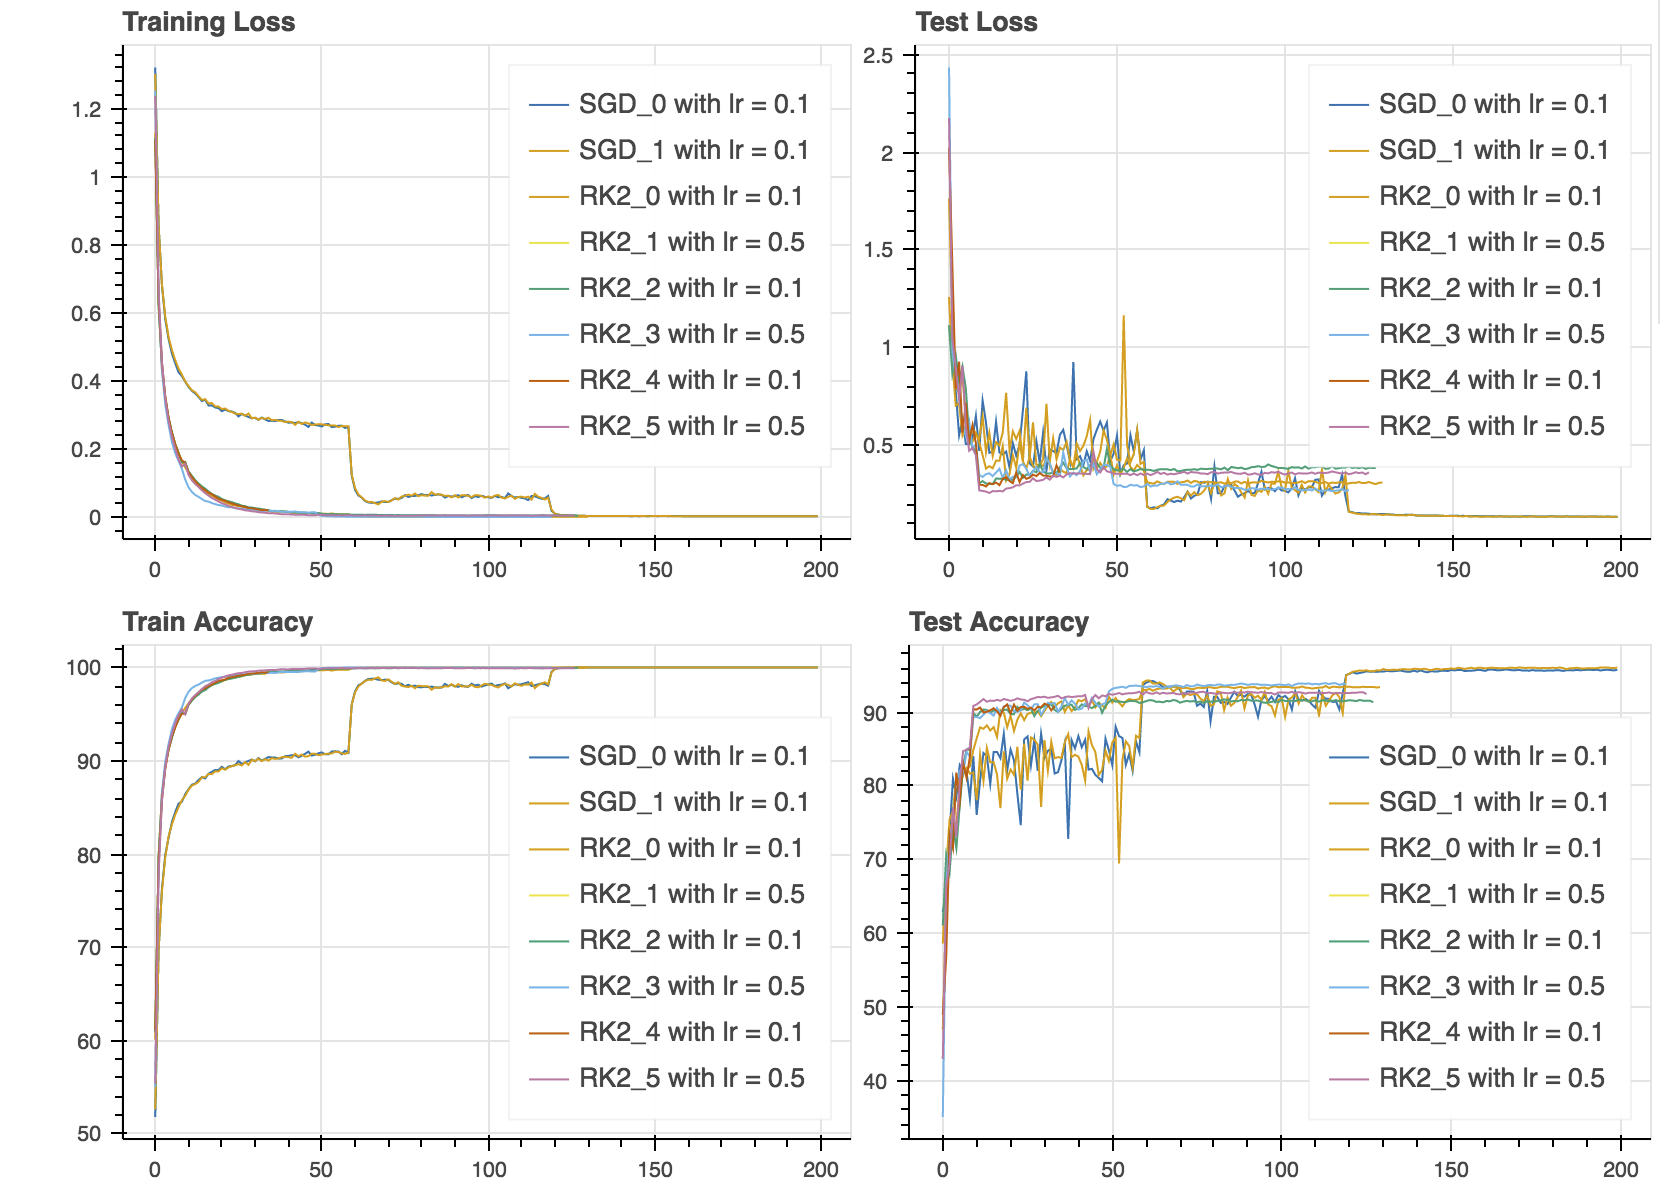
\includegraphics[scale=0.5]{wideresnet.png}

\subsection{Convex Models}


\end{document}

%%% Local Variables:
%%% mode: latex
%%% TeX-master: t
%%% End:
